%package list
\documentclass{article}
\usepackage[top=3cm, bottom=3cm, outer=3cm, inner=3cm]{geometry}
\usepackage{multicol}
\usepackage{graphicx}
\usepackage{url}
%\usepackage{cite}
\usepackage{hyperref}
\usepackage{array}
%\usepackage{multicol}
\newcolumntype{x}[1]{>{\centering\arraybackslash\hspace{0pt}}p{#1}}
\usepackage{natbib}
\usepackage{pdfpages}
\usepackage{multirow}
\usepackage[normalem]{ulem}
\useunder{\uline}{\ul}{}
\usepackage{svg}
\usepackage{xcolor}
\usepackage{listings}
\lstdefinestyle{ascii-tree}{
    literate={├}{|}1 {─}{--}1 {└}{+}1 
  }
\lstset{basicstyle=\ttfamily,
  showstringspaces=false,
  commentstyle=\color{red},
  keywordstyle=\color{blue}
}
%\usepackage{booktabs}
\usepackage{caption}
\usepackage{subcaption}
\usepackage{float}
\usepackage{array}

\usepackage{enumitem}


\newcolumntype{M}[1]{>{\centering\arraybackslash}m{#1}}
\newcolumntype{N}{@{}m{0pt}@{}}


%%%%%%%%%%%%%%%%%%%%%%%%%%%%%%%%%%%%%%%%%%%%%%%%%%%%%%%%%%%%%%%%%%%%%%%%%%%%
%%%%%%%%%%%%%%%%%%%%%%%%%%%%%%%%%%%%%%%%%%%%%%%%%%%%%%%%%%%%%%%%%%%%%%%%%%%%
\newcommand{\itemEmail}{vmaldonadov@unsa.edu.pe}
\newcommand{\itemStudent}{Victor Gonzalo Maldonado Vilca}
\newcommand{\itemCourse}{Programación Web 2}
\newcommand{\itemCourseCode}{1702122}
\newcommand{\itemSemester}{III}
\newcommand{\itemUniversity}{Universidad Nacional de San Agustín de Arequipa}
\newcommand{\itemFaculty}{Facultad de Ingeniería de Producción y Servicios}
\newcommand{\itemDepartment}{Departamento Académico de Ingeniería de Sistemas e Informática}
\newcommand{\itemSchool}{Escuela Profesional de Ingeniería de Sistemas}
\newcommand{\itemAcademic}{2024 - A}
\newcommand{\itemInput}{Del 9 de abril de 2024}
\newcommand{\itemOutput}{Al 15 de mayo de 2024}
\newcommand{\itemPracticeNumber}{03}
\newcommand{\itemTheme}{JavaScript}
%%%%%%%%%%%%%%%%%%%%%%%%%%%%%%%%%%%%%%%%%%%%%%%%%%%%%%%%%%%%%%%%%%%%%%%%%%%%
%%%%%%%%%%%%%%%%%%%%%%%%%%%%%%%%%%%%%%%%%%%%%%%%%%%%%%%%%%%%%%%%%%%%%%%%%%%%

\usepackage[english,spanish]{babel}
\usepackage[utf8]{inputenc}
\AtBeginDocument{\selectlanguage{spanish}}
\renewcommand{\figurename}{Figura}
\renewcommand{\refname}{Referencias}
\renewcommand{\tablename}{Tabla} %esto no funciona cuando se usa babel
\AtBeginDocument{%
	\renewcommand\tablename{Tabla}
}

\usepackage{fancyhdr}
\pagestyle{fancy}
\fancyhf{}
\setlength{\headheight}{30pt}
\renewcommand{\headrulewidth}{1pt}
\renewcommand{\footrulewidth}{1pt}
\fancyhead[L]{\raisebox{-0.2\height}{
\includegraphics[width=3cm]{img/logo_episunsa.png}}}
\fancyhead[C]{\fontsize{7}{7}\selectfont	\itemUniversity \\ \itemFaculty \\ \itemDepartment \\ \itemSchool \\ \textbf{\itemCourse}}
\fancyhead[R]{\raisebox{-0.2\height}{
\includegraphics[width=1.2cm]{img/logo_abet}}}
\fancyfoot[L]{Victor M.}
\fancyfoot[C]{\itemCourse}
\fancyfoot[R]{Página \thepage}

% para el codigo fuente
\usepackage{listings}
\usepackage{color, colortbl}
\definecolor{dkgreen}{rgb}{0,0.6,0}
\definecolor{gray}{rgb}{0.5,0.5,0.5}
\definecolor{mauve}{rgb}{0.58,0,0.82}
\definecolor{codebackground}{rgb}{0.95, 0.95, 0.92}
\definecolor{tablebackground}{rgb}{0.8, 0, 0}

\lstset{frame=tb,
	language=bash,
	aboveskip=3mm,
	belowskip=3mm,
	showstringspaces=false,
	columns=flexible,
	basicstyle={\small\ttfamily},
	numbers=none,
	numberstyle=\tiny\color{gray},
	keywordstyle=\color{blue},
	commentstyle=\color{dkgreen},
	stringstyle=\color{mauve},
	breaklines=true,
	breakatwhitespace=true,
	tabsize=3,
	backgroundcolor= \color{codebackground},
}

\begin{document}
	
	\vspace*{10px}
	
	\begin{center}	
		\fontsize{17}{17} \textbf{ Informe de Laboratorio 03}
	\end{center}
	\centerline{\textbf{\Large Tema: \itemTheme}}
	%\vspace*{0.5cm}	

	\begin{flushright}
		\begin{tabular}{|M{2.5cm}|N|}
			\hline 
			\rowcolor{tablebackground}
			\color{white} \textbf{Nota}  \\
			\hline 
			     \\[30pt]
			\hline 			
		\end{tabular}
	\end{flushright}	

	\begin{table}[H]
		\begin{tabular}{|x{4.7cm}|x{4.8cm}|x{4.8cm}|}
			\hline 
			\rowcolor{tablebackground}
			\color{white} \textbf{Estudiante} & \color{white}\textbf{Escuela}  & \color{white}\textbf{Asignatura}   \\
			\hline 
			{\itemStudent \par \itemEmail} & \itemSchool & {\itemCourse \par Semestre: \itemSemester \par Código: \itemCourseCode}     \\
			\hline 			
		\end{tabular}
	\end{table}		
	
	\begin{table}[H]
		\begin{tabular}{|x{4.7cm}|x{4.8cm}|x{4.8cm}|}
			\hline 
			\rowcolor{tablebackground}
			\color{white}\textbf{Tarea} & \color{white}\textbf{Tema}  & \color{white}\textbf{Duración}   \\
			\hline 
			\itemPracticeNumber & \itemTheme & 2 horas   \\
			\hline 
		\end{tabular}
	\end{table}
	
	\begin{table}[H]
		\begin{tabular}{|x{4.7cm}|x{4.8cm}|x{4.8cm}|}
			\hline 
			\rowcolor{tablebackground}
			\color{white}\textbf{Semestre académico} & \color{white}\textbf{Fecha de inicio}  & \color{white}\textbf{Fecha de entrega}   \\
			\hline 
			\itemAcademic & \itemInput &  \itemOutput  \\
			\hline 
		\end{tabular}
	\end{table}
	

%%%%%%%%%%%%%%%%%%%%
 
	\section{Tarea}
	\textbf{Ejercicios Propuestos:}
	\begin{itemize}		
		\item Escriba una función que reciba el número de día de la fecha actual new Date()  y devuelva el texto del día de la semana correspondientes. Por ejemplo si recibe 0, devolvería “Domingo”.
        \item Escriba una página web que reciba un texto y al presionar un botón muestre el mismo texto invertido en otra sección (div). Por ejemplo si se escribe “Hola”, se mostraría como “aloH”.
        \item Escribir una página que muestre cuántos días faltan para el día de Arequipa!
        \item Escribir un página que reciba el URL de la sesión de google meet de hoy y devuelva el código de la sesión sin guiones separadores.
        \item Escribir una página que permita calcular la suma de todos los valores de una tabla de valores dinámica. La idea es crear una página web con un formulario que te permita decir cuantos valores tendrá la tabla, luego, al enviar el formulario la tabla se debe crear dinámica y aleatoriamente, junto con otro botón de envió para calcular la suma.
        \item En su tarea deberán implementar las siguientes páginas.
        \begin{itemize}
        	\item Pagina1.html - Cree una página web con un texto y dos botones (al estilo del ejemplo del foco que se enciende y apaga) que permitan cambiar el tamaño de la letra de un texto, intente hacerlo también con los colores.
        	\item Pagina2.html - Cree una página web que permita realizar las operaciones aritmética, lógicas y de bits básicas, de manera dinámica( se podrá elegir cualquier operador) y se trabajará con dos argumentos.
        \end{itemize}
        \item Resolver los 67 ejercicios de javaScript en w3schools.com y subir un pantallazo con su nombre y apellido.
	\end{itemize}
 
    \section{Entregables}
    \begin{itemize}
        \item Informe de trabajo
        \item URL: Repositorio de GitHub
        \item URL: Vídeo en Youtube
    \end{itemize}
    
		
	\section{Equipos, materiales y temas utilizados}
	\begin{itemize}
		\item HTML
		\item CSS
		\item JavaScript
		\item w3schools
        \item GitHub
        
	\end{itemize}
 
	
	\section{URL de Repositorio Github}
	\begin{itemize}
		\item URL del Repositorio GitHub para clonar o recuperar.
		\item \url{https://github.com/Victor-Gonzalo-Maldonado-Vilca/pw2-lab03.git}
	\end{itemize}

%%%%%%%%%%%%%%%%%%%%
	\section{URL de Vídeo en Youtube}
	\begin{itemize}
		\item URL de youtube, donde estará el video explicativo de los ejercicios.
		\item \url{https://www.youtube.com/watch?v=-BQzJIAwX4s}
	\end{itemize}
%%%%%%%%%%%%%%%%%%%%


    \section{Desarrollo del trabajo}
    \subsection{Ejercicio 1}
    \begin{itemize}
    	\item Colocando en un Array los valores de los días, mediante la presente funccion que recibira como parámetro un entero se logrará retornar un string que sera el día correspondiente. 
    	\lstinputlisting[language=JavaScript, firstline=1, lastline=8, firstnumber=1, caption={Script 1 - parte 1},numbers=left,]{../Ejercicios_Propuestos/Ejercicio_1/Ejercicio1.js}
    	\newpage
    	\item Extrayendo el día actual usando la clase Date y sus métodos correspondientes, además se llama a la anterior funcción
    	\lstinputlisting[language=JavaScript, firstline=9, lastline=11, firstnumber=9, caption={Script 1 - parte 2},numbers=left,]{../Ejercicios_Propuestos/Ejercicio_1/Ejercicio1.js}
    \end{itemize}
    \subsubsection{Ejecución}
    \begin{figure}[H]
    	\centering
    	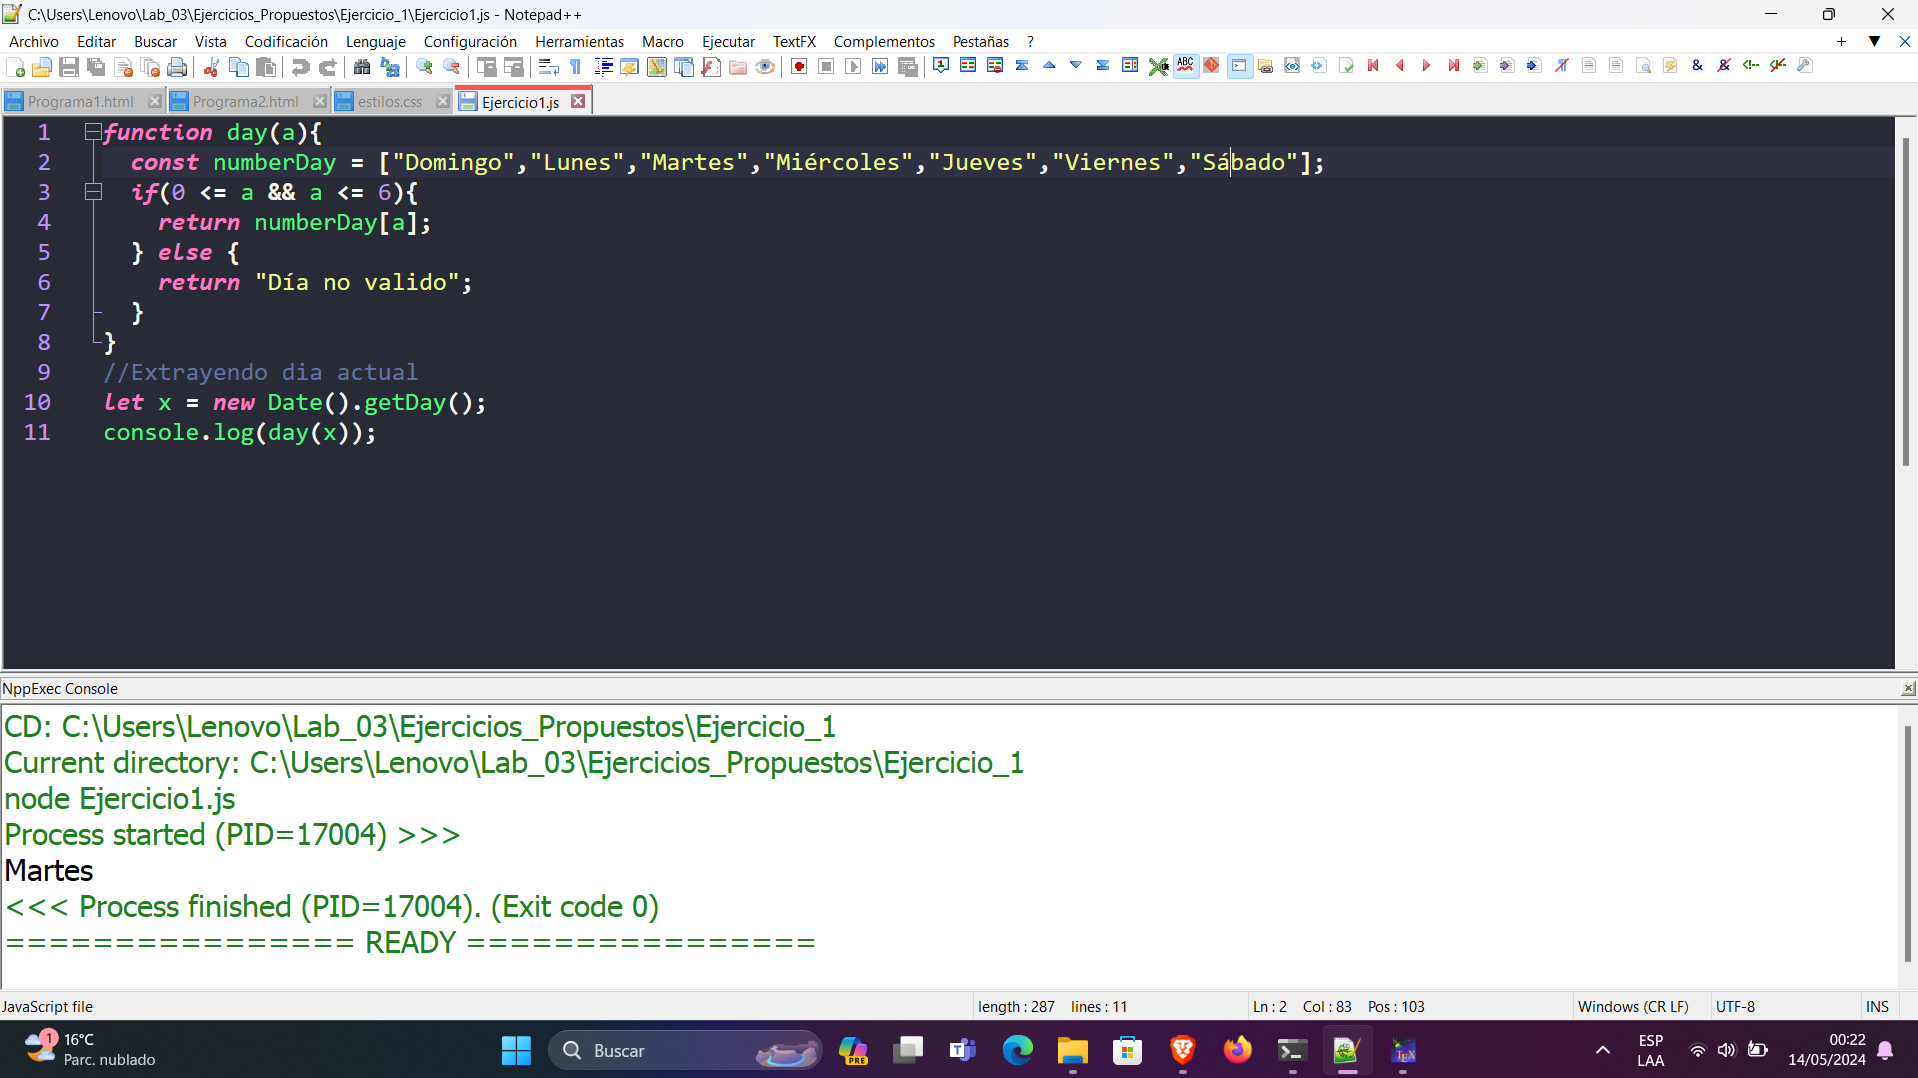
\includegraphics[width=1\textwidth,keepaspectratio]{img/EScript1.png}
    	\caption{Ejecución - Ejercicio 1}
    \end{figure}
    
%%%%%%%%%%%%%%%%%%%%
	\subsection{Ejercicio 2}
	\subsubsection{HTML}
	\begin{itemize}
		\item Etiqueta head donde se encontrarán las etiquetas meta, el título y los estilos  
		\lstinputlisting[language=HTML, firstline=3, lastline=8, firstnumber=3, caption={HTML - parte 1},numbers=left,]{../Ejercicios_Propuestos/Ejercicio_2/Ejercicio2.html}
		\newpage
		\item Agregar un formulario para obtener el texto que ingrese el usuario
		\lstinputlisting[language=HTML, firstline=12, lastline=17, firstnumber=12, caption={HTML - parte 2},numbers=left,]{../Ejercicios_Propuestos/Ejercicio_2/Ejercicio2.html}
		\item Este código JavaScript escucha el evento de envío de un formulario ('submit'). Al recibir este evento, evita la acción predeterminada, invierte una cadena de texto ingresada por el usuario y muestra el resultado en la página web.
		\lstinputlisting[language=HTML, firstline=24, lastline=33, firstnumber=24, caption={Script 2},numbers=left,]{../Ejercicios_Propuestos/Ejercicio_2/Ejercicio2.html}
	\end{itemize}
	\subsubsection{CSS}
	\begin{itemize}
		\item Agregar estilos a la página.
		\lstinputlisting[language=CSS, firstline=1, lastline=38, firstnumber=1, caption={Estilos},numbers=left,]{../Ejercicios_Propuestos/Ejercicio_2/css/estilos.css}
	\end{itemize}
	\subsubsection{Ejecución}
	\begin{figure}[H]
		\centering
		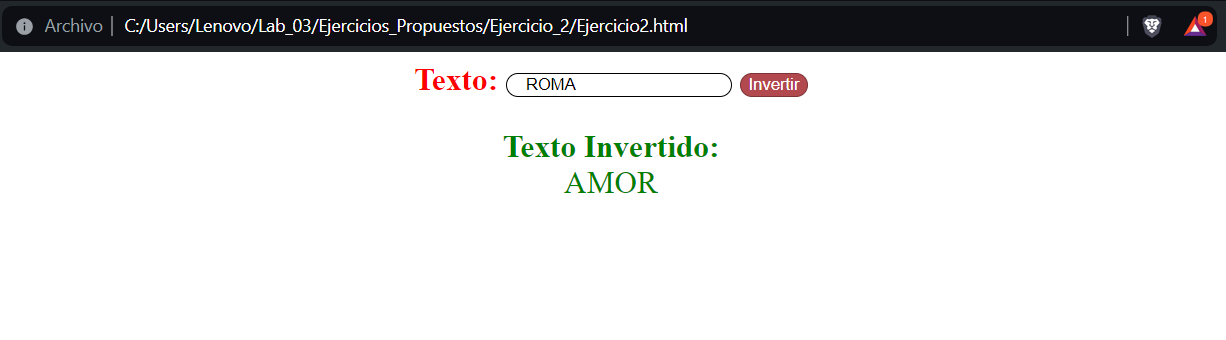
\includegraphics[width=1\textwidth,keepaspectratio]{img/HTML1.png}
		\caption{Ejecución - Ejercicio 2}
	\end{figure}
%%%%%%%%%%%%%%%%%%%%
	\subsection{Ejercicio 3}
	\subsubsection{HTML}
	\begin{itemize}
		\item Etiqueta head donde se encontrarán las etiquetas meta, el título y los estilos  
		\lstinputlisting[language=HTML, firstline=3, lastline=8, firstnumber=3, caption={HTML - parte 1},numbers=left,]{../Ejercicios_Propuestos/Ejercicio_3/Ejercicio3.html}
		\newpage
		\item Agregar un formulario para poder realizar un evento al presionar el botón
		\lstinputlisting[language=HTML, firstline=12, lastline=15, firstnumber=12, caption={HTML - parte 2},numbers=left,]{../Ejercicios_Propuestos/Ejercicio_3/Ejercicio3.html}
		\item En esta parte, es donde mediante con el script se logrará colocar la respuesta correcta, en este caso los días que faltan para el día de Arequipa. 
		\lstinputlisting[language=HTML, firstline=18, lastline=20, firstnumber=18, caption={HTML - parte 3},numbers=left,]{../Ejercicios_Propuestos/Ejercicio_3/Ejercicio3.html}
		\item Este script JavaScript captura el evento de envío de un formulario con el ID "formulario". Al recibir este evento, calcula la diferencia en días entre una fecha específica ('2024-08-15') y la fecha actual. Luego, muestra esta diferencia de días en un elemento del documento con el ID "fecha".
		\lstinputlisting[language=HTML, firstline=21, lastline=32, firstnumber=21, caption={Script 3},numbers=left,]{../Ejercicios_Propuestos/Ejercicio_3/Ejercicio3.html}
	\end{itemize}
		\subsubsection{CSS}
	\begin{itemize}
		\item Agregar estilos a la página.
		\lstinputlisting[language=CSS, firstline=1, lastline=24, firstnumber=1, caption={Estilos},numbers=left,]{../Ejercicios_Propuestos/Ejercicio_3/css/estilos.css}
	\end{itemize}
	\subsubsection{Ejecución}
	\begin{figure}[H]
		\centering
		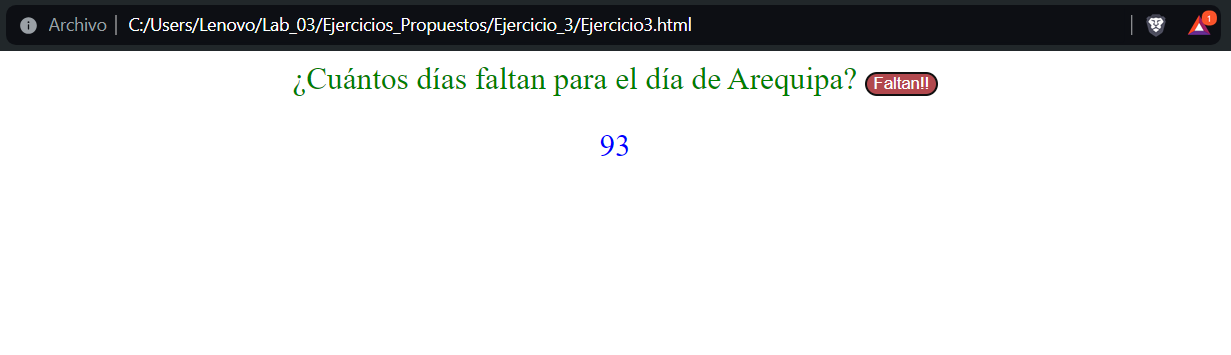
\includegraphics[width=1\textwidth,keepaspectratio]{img/HTML2.png}
		\caption{Ejecución - Ejercicio 3}
	\end{figure}
%%%%%%%%%%%%%%%%%%%%
	\subsection{Ejercicio 4}
	\subsubsection{HTML}
	\begin{itemize}
		\item Etiqueta head donde se encontrarán las etiquetas meta, el título y los estilos  
		\lstinputlisting[language=HTML, firstline=3, lastline=8, firstnumber=3, caption={HTML - parte 1},numbers=left,]{../Ejercicios_Propuestos/Ejercicio_4/Ejercicio4.html}
		\newpage
		\item Agregar un formulario donde el usuario colocara el enlace meet.
		\lstinputlisting[language=HTML, firstline=11, lastline=15, firstnumber=11, caption={HTML - parte 2},numbers=left,]{../Ejercicios_Propuestos/Ejercicio_4/Ejercicio4.html}
		\item En esta parte, es donde mediante con el script se logrará colocar la respuesta correcta, en este caso el código del enlace meet. 
		\lstinputlisting[language=HTML, firstline=17, lastline=20, firstnumber=17, caption={HTML - parte 3},numbers=left,]{../Ejercicios_Propuestos/Ejercicio_4/Ejercicio4.html}
		\item Este script JavaScript captura el envío de un formulario y evita su acción predeterminada. Extrae un código específico de una URL ingresada por el usuario, eliminando los primeros 24 caracteres y los guiones. Luego, muestra este código en la página.
		\lstinputlisting[language=HTML, firstline=21, lastline=35, firstnumber=21, caption={Script 4},numbers=left,]{../Ejercicios_Propuestos/Ejercicio_4/Ejercicio4.html}
	\end{itemize}
	\subsubsection{CSS}
	\begin{itemize}
		\item Agregar estilos a la página.
		\lstinputlisting[language=CSS, firstline=1, lastline=42, firstnumber=1, caption={Estilos},numbers=left,]{../Ejercicios_Propuestos/Ejercicio_4/css/estilos.css}
	\end{itemize}
	\subsubsection{Ejecución}
	\begin{figure}[H]
		\centering
		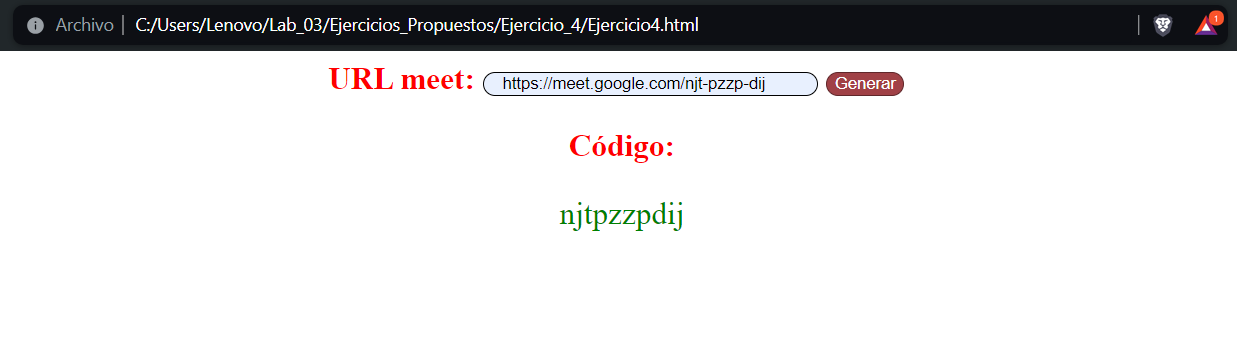
\includegraphics[width=1\textwidth,keepaspectratio]{img/HTML3.png}
		\caption{Ejecución - Ejercicio 4}
	\end{figure}
	\newpage
%%%%%%%%%%%%%%%%%%%%
	\subsection{Ejercicio 5}
	\subsubsection{HTML}
	\begin{itemize}
		\item Etiqueta head donde se encontrarán las etiquetas meta, el título y los estilos  
		\lstinputlisting[language=HTML, firstline=3, lastline=7, firstnumber=3, caption={HTML - parte 1},numbers=left,]{../Ejercicios_Propuestos/Ejercicio_5/Ejercicio5.html}
		\item Agregar un formulario donde el usuario colocara una cantidad, para que se cree una tabla con valores númericos aleatorios en cada celda.
		\lstinputlisting[language=HTML, firstline=11, lastline=15, firstnumber=11, caption={HTML - parte 2},numbers=left,]{../Ejercicios_Propuestos/Ejercicio_5/Ejercicio5.html}
		\item En esta parte, es donde mediante con el script se logrará colocar la respuesta correcta, en este caso tanto la tabla como la suma.
		\lstinputlisting[language=HTML, firstline=17, lastline=20, firstnumber=17, caption={HTML - parte 3},numbers=left,]{../Ejercicios_Propuestos/Ejercicio_5/Ejercicio5.html}
		\item Este script en JavaScript captura el envío de un formulario y evita su acción predeterminada. Luego, crea una tabla con números aleatorios en filas de 50 elementos cada una, basada en la cantidad ingresada por el usuario. Finalmente, agrega un botón "Sumar" para realizar una acción adicional al hacer clic en él.
		\lstinputlisting[language=HTML, firstline=21, lastline=45, firstnumber=21, caption={Script 5 - parte 1},numbers=left,]{../Ejercicios_Propuestos/Ejercicio_5/Ejercicio5.html}
		\item La función suma los valores numéricos de una tabla en la página web y muestra el resultado en verde en el elemento con el ID "resultado".
		\lstinputlisting[language=HTML, firstline=46, lastline=56, firstnumber=46, caption={Script 5 - parte 2},numbers=left,]{../Ejercicios_Propuestos/Ejercicio_5/Ejercicio5.html}
	\end{itemize}
	\subsubsection{CSS}
	\begin{itemize}
		\item Agregar estilos a la página.
		\lstinputlisting[language=CSS, firstline=1, lastline=28, firstnumber=1, caption={Estilos},numbers=left,]{../Ejercicios_Propuestos/Ejercicio_5/css/estilos.css}
	\end{itemize}
	\subsubsection{Ejecución}
	\begin{figure}[H]
		\centering
		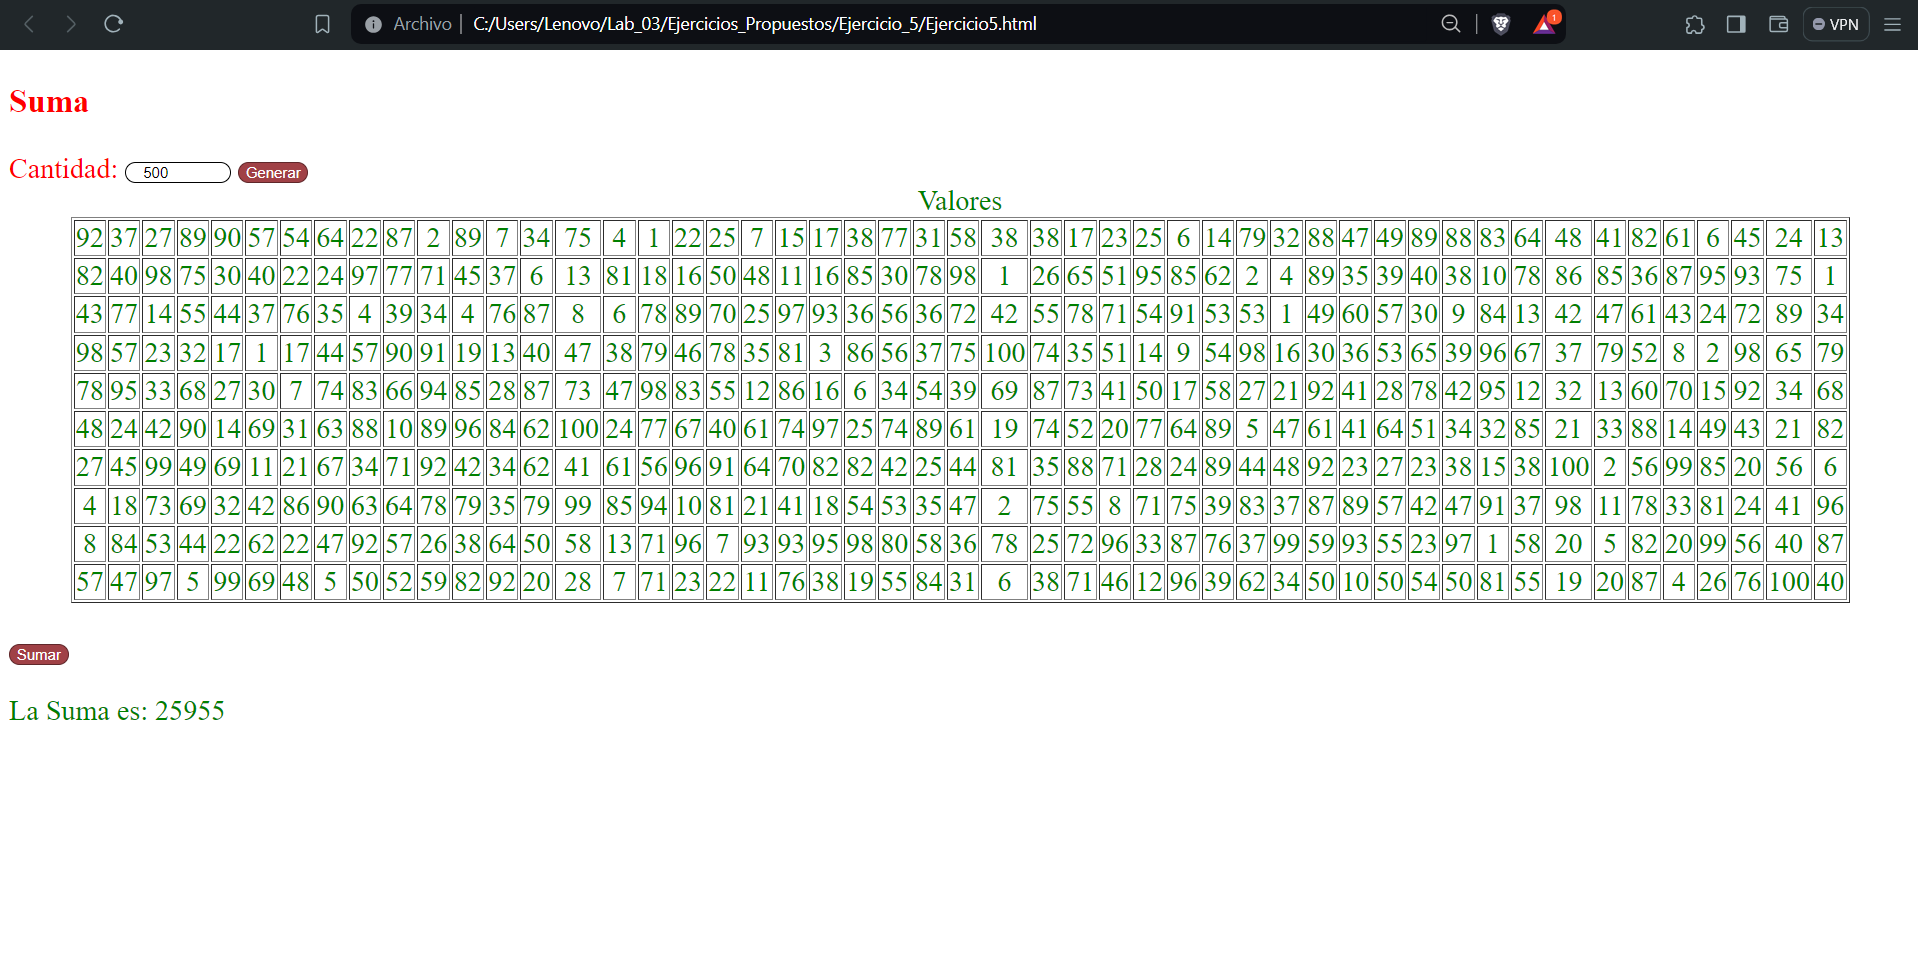
\includegraphics[width=1\textwidth,keepaspectratio]{img/HTML4.png}
		\caption{Ejecución - Ejercicio 5}
	\end{figure}
	
%%%%%%%%%%%%%%%%%%%%
	
	\subsection{Ejercicio 6 - Programa 1}
	\subsubsection{HTML}
	\begin{itemize}
		\item Etiqueta head donde se encontrarán las etiquetas meta, el título y los estilos  
		\lstinputlisting[language=HTML, firstline=3, lastline=7, firstnumber=3, caption={HTML - parte 1},numbers=left,]{../Ejercicios_Propuestos/Ejercicio_6/Programa1.html}
		\newpage
		\item Crear botones con atributos onclick que cambiaran el tamaño y color del texto.
		\lstinputlisting[language=HTML, firstline=9, lastline=17, firstnumber=9, caption={HTML - parte 2},numbers=left,]{../Ejercicios_Propuestos/Ejercicio_6/Programa1.html}
		\item El script JavaScript cambia dinámicamente el tamaño y el color del texto en un elemento específico de una página web, usando funciones de por medio que manipulan los elementos del HTML, en este caso el texto.
		\lstinputlisting[language=HTML, firstline=18, lastline=31, firstnumber=18, caption={Script 6 - programa 1},numbers=left,]{../Ejercicios_Propuestos/Ejercicio_6/Programa1.html}
	\end{itemize}
	\subsubsection{Ejecución}
	\begin{figure}[H]
		\centering
		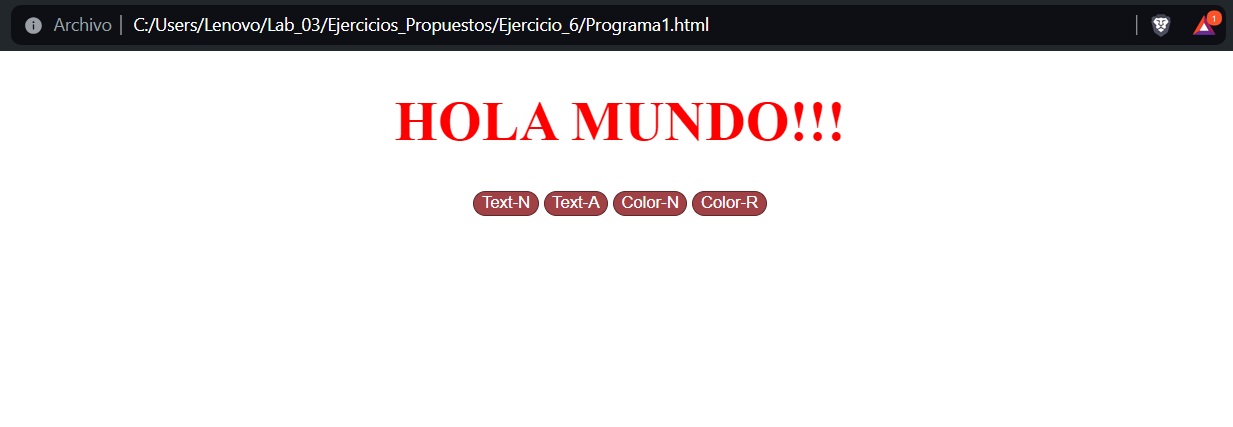
\includegraphics[width=1\textwidth,keepaspectratio]{img/HTML5.png}
		\caption{Ejecución - Ejercicio 6 P1}
	\end{figure}
%%%%%%%%%%%%%%%%%%%%
	\subsection{Ejercicio 6 - Programa 2}
	\subsubsection{HTML}
	\begin{itemize}
		\item Etiqueta head donde se encontrarán las etiquetas meta, el título y los estilos  
		\lstinputlisting[language=HTML, firstline=3, lastline=7, firstnumber=3, caption={HTML - parte 1},numbers=left,]{../Ejercicios_Propuestos/Ejercicio_6/Programa2.html}
		\item Implementar un formulario que pedirá al usuario dos numeros y un operador que se calculará mas adelante.
		\lstinputlisting[language=HTML, firstline=10, lastline=39, firstnumber=10, caption={HTML - parte 2},numbers=left,]{../Ejercicios_Propuestos/Ejercicio_6/Programa2.html}
		\item En esta parte, es donde mediante con el script se logrará colocar la respuesta correcta, en este caso el cálculo de los números , con el operador correspondiente.
		\lstinputlisting[language=HTML, firstline=41, lastline=42, firstnumber=41, caption={HTML - parte 3},numbers=left,]{../Ejercicios_Propuestos/Ejercicio_6/Programa2.html}
		\item El script JavaScript captura el envío de un formulario, evita su acción predeterminada y calcula el resultado de una operación matemática basada en los números y el operador seleccionados por el usuario. El resultado se muestra en la página.
		\lstinputlisting[language=HTML, firstline=43, lastline=93, firstnumber=43, caption={Script 6 - Programa 2},numbers=left,]{../Ejercicios_Propuestos/Ejercicio_6/Programa2.html}
	\end{itemize}
	\subsubsection{Ejecución}
	\begin{figure}[H]
		\centering
		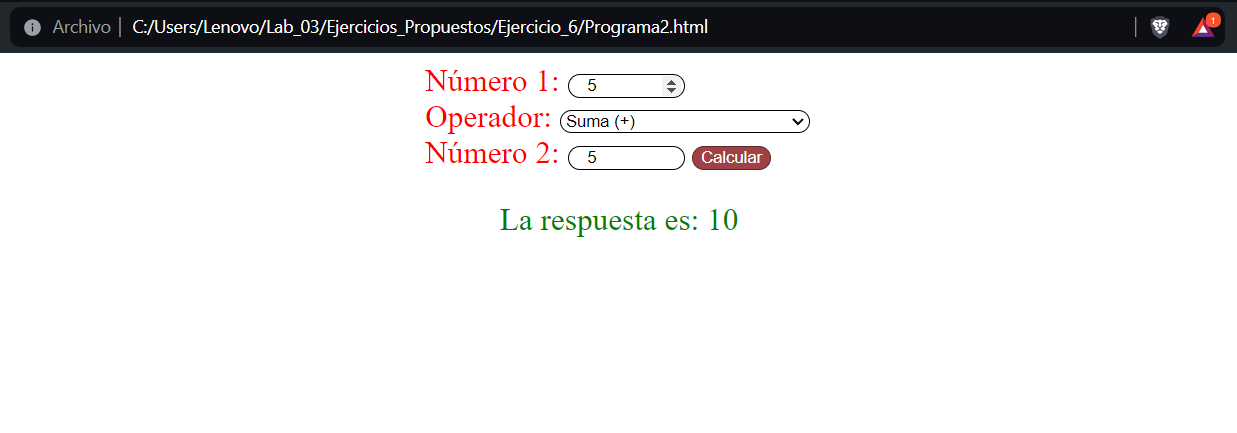
\includegraphics[width=1\textwidth,keepaspectratio]{img/suma.png}
		\caption{Ejecución - Suma}
	\end{figure}
	\begin{figure}[H]
		\centering
		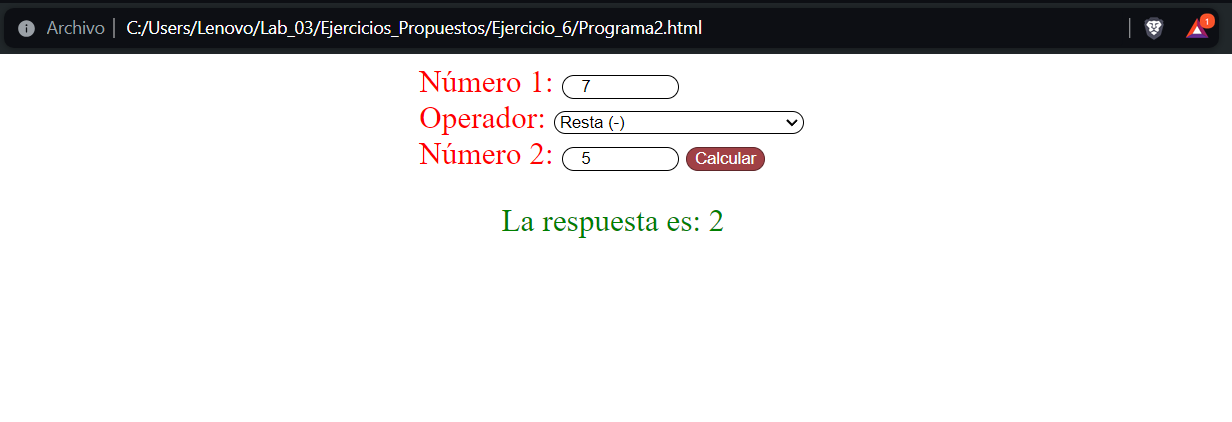
\includegraphics[width=1\textwidth,keepaspectratio]{img/resta.png}
		\caption{Ejecución - Resta}
	\end{figure}
	\begin{figure}[H]
		\centering
		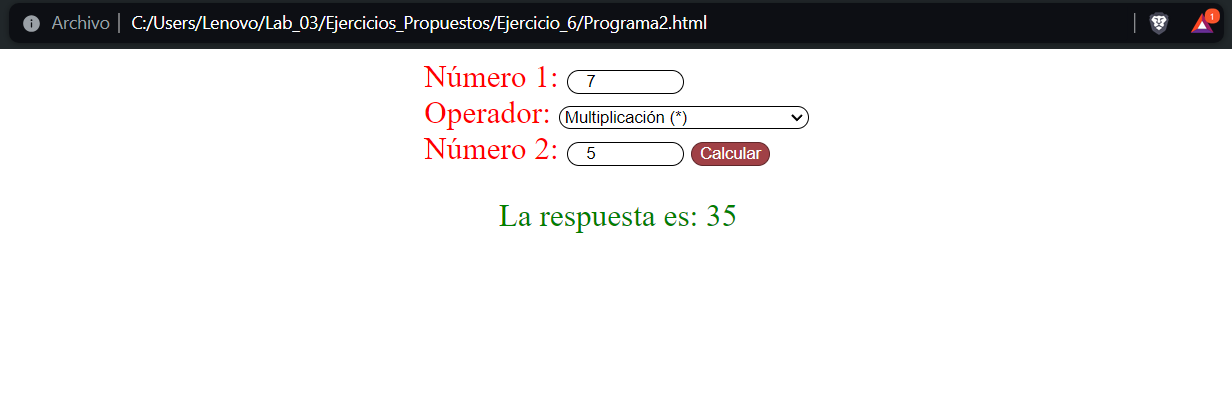
\includegraphics[width=1\textwidth,keepaspectratio]{img/multi.png}
		\caption{Ejecución - Multiplicación}
	\end{figure}
	\begin{figure}[H]
		\centering
		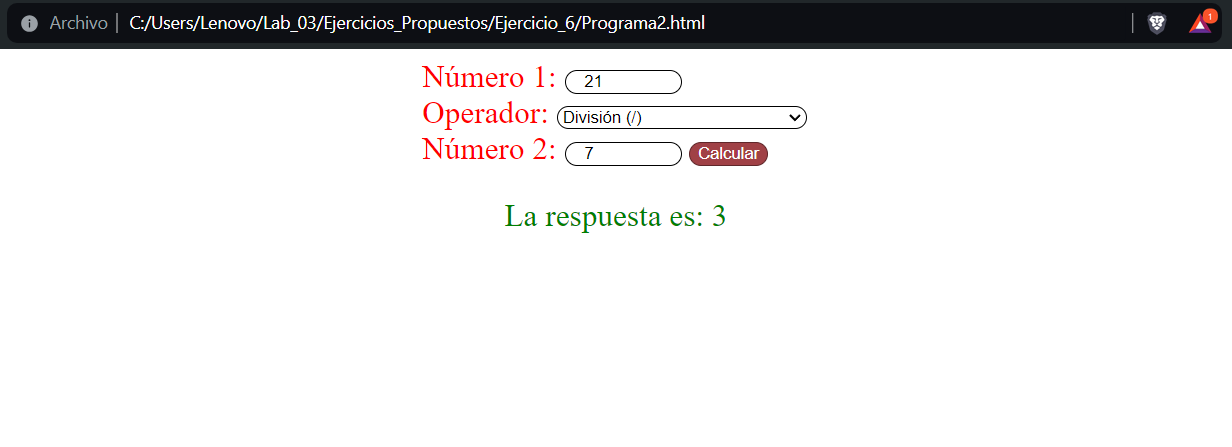
\includegraphics[width=1\textwidth,keepaspectratio]{img/div.png}
		\caption{Ejecución - División}
	\end{figure}
	\begin{figure}[H]
		\centering
		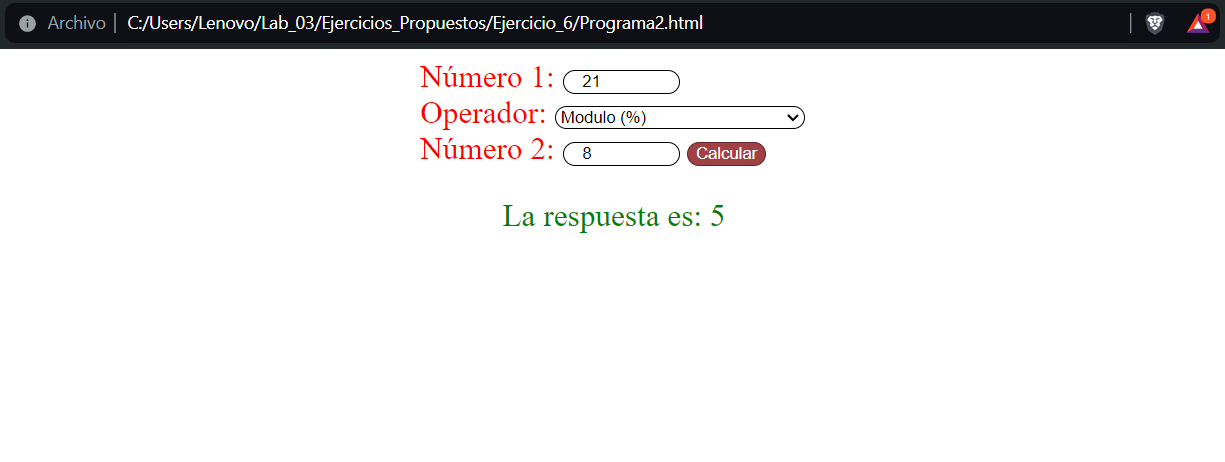
\includegraphics[width=1\textwidth,keepaspectratio]{img/mod.png}
		\caption{Ejecución - Modulo}
	\end{figure}
	\begin{figure}[H]
		\centering
		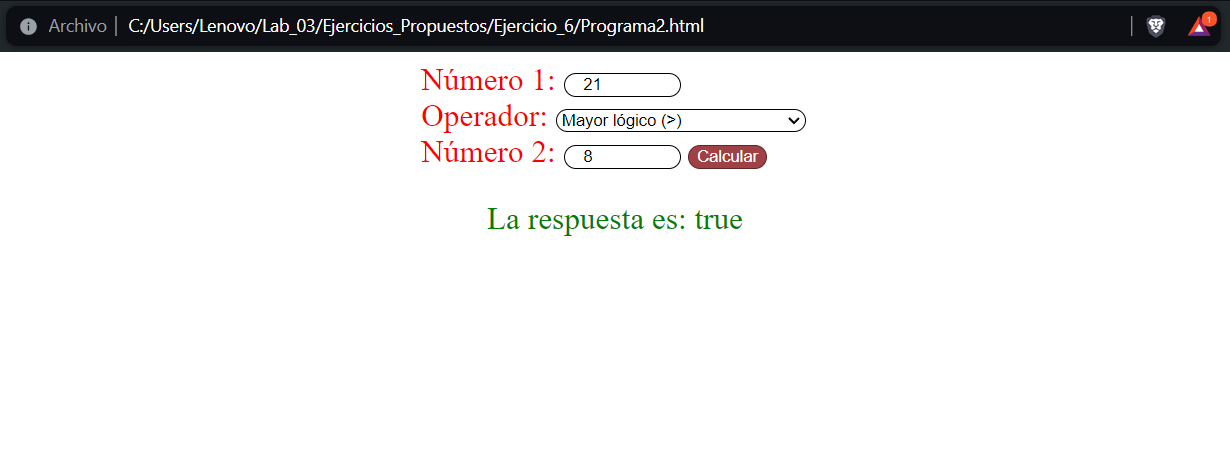
\includegraphics[width=1\textwidth,keepaspectratio]{img/may.png}
		\caption{Ejecución - Mayor}
	\end{figure}
	\begin{figure}[H]
		\centering
		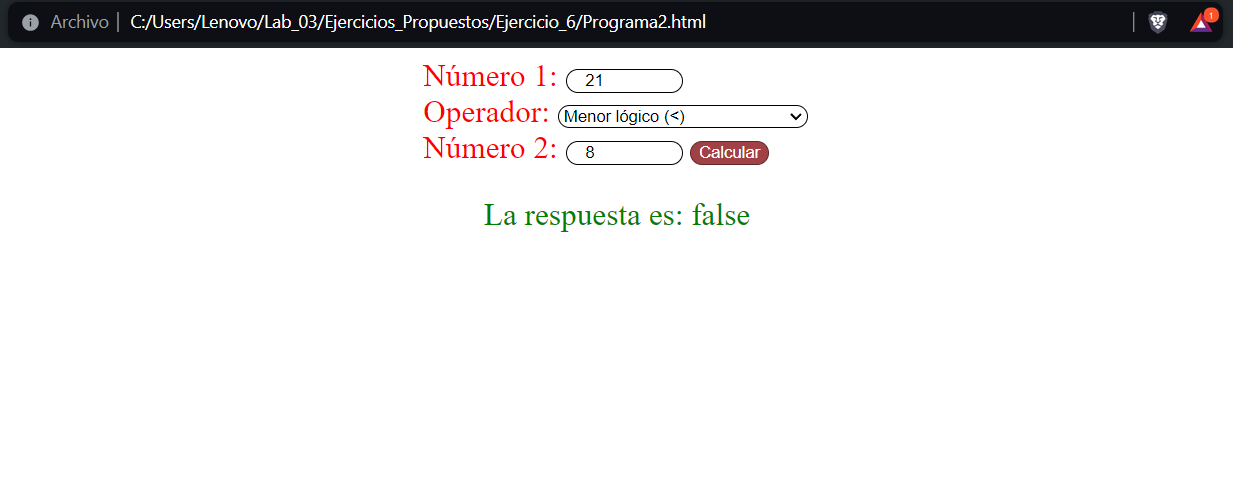
\includegraphics[width=1\textwidth,keepaspectratio]{img/men.png}
		\caption{Ejecución - Menor}
	\end{figure}
	\textbf{CSS de los dos programas: }
	\lstinputlisting[language=CSS, firstline=1, lastline=38, firstnumber=1, caption={Estilos},numbers=left,]{../Ejercicios_Propuestos/Ejercicio_6/css/estilos.css}
%%%%%%%%%%%%%%%%%%%%
	\subsection{Ejercicios w3schools}
	\begin{figure}[H]
		\centering
		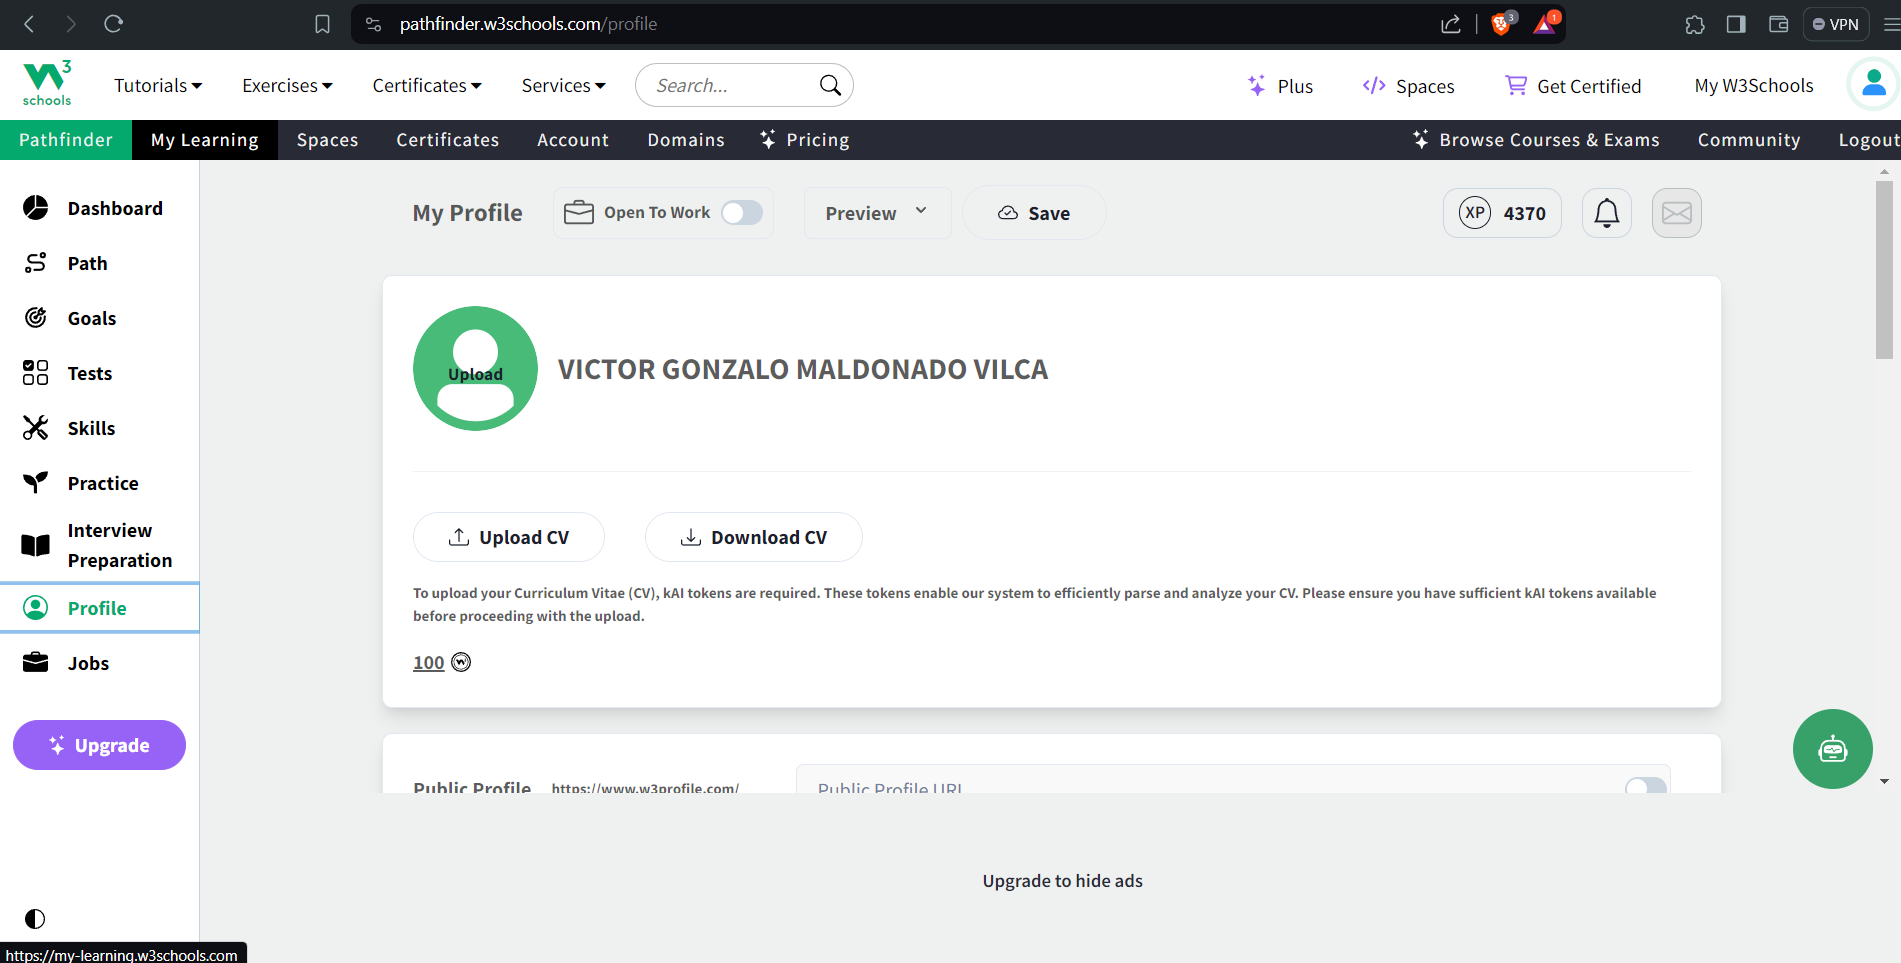
\includegraphics[width=1\textwidth,keepaspectratio]{img/w3_user.png}
		\caption{Usuario - w3schools}
	\end{figure}
	\begin{figure}[H]
		\centering
		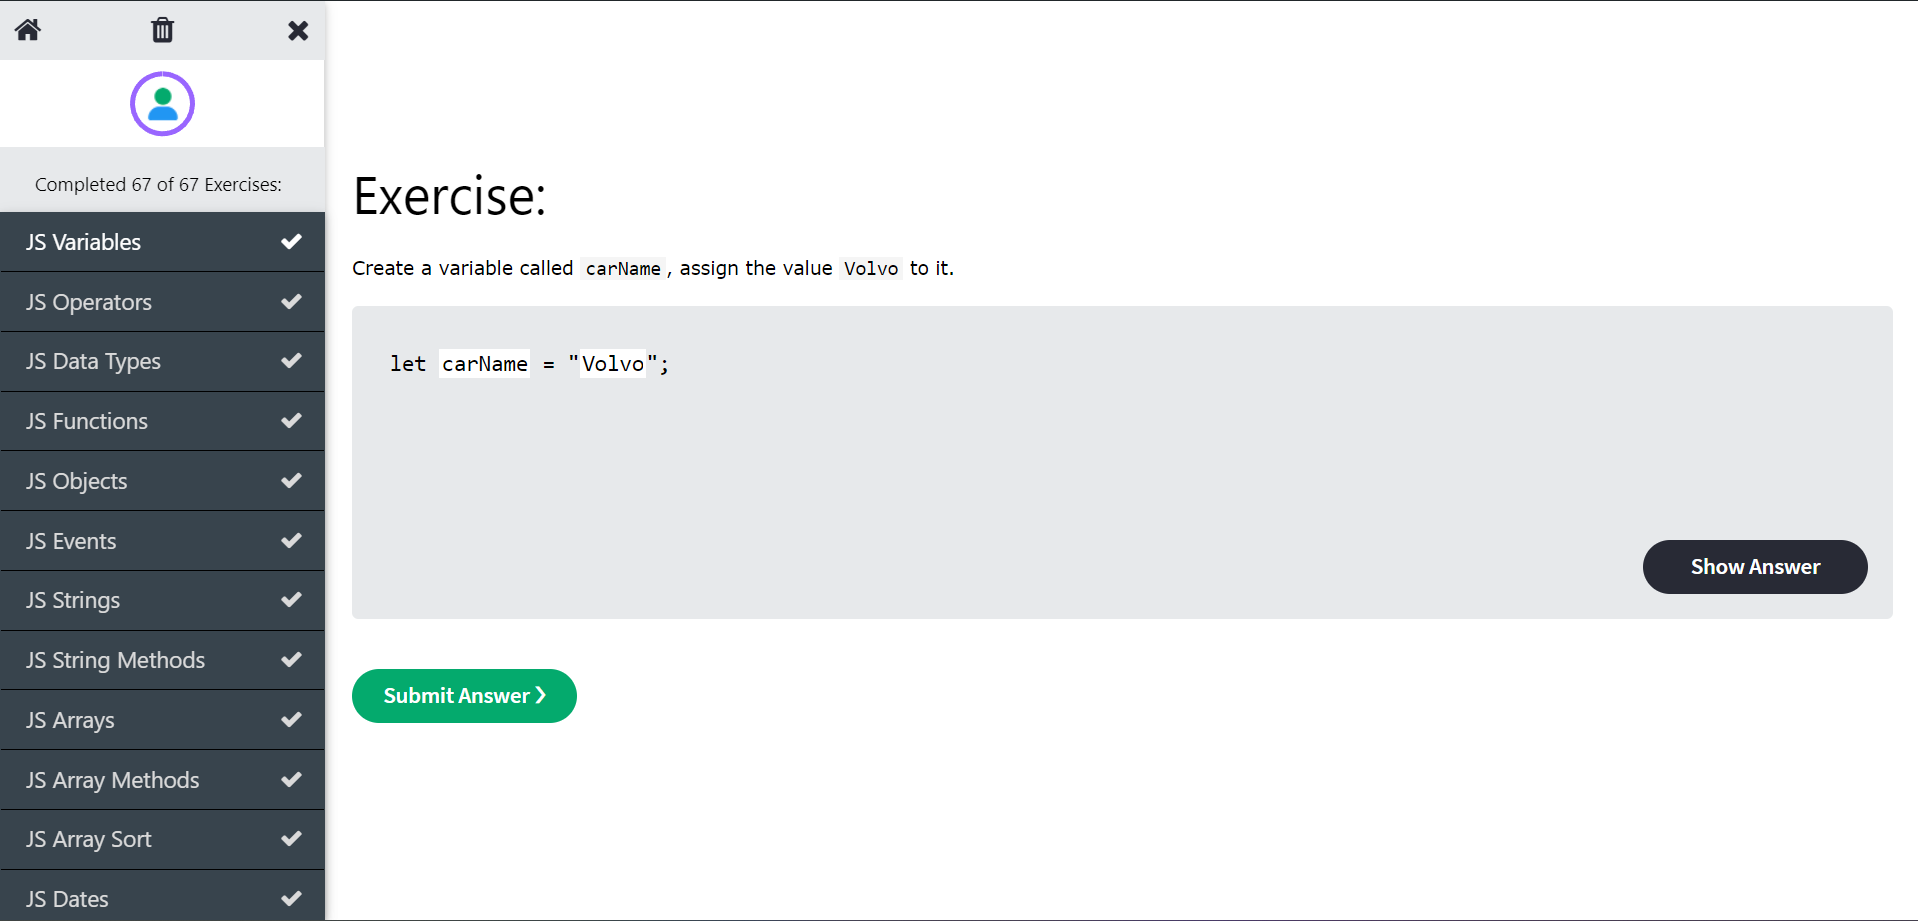
\includegraphics[width=1\textwidth,keepaspectratio]{img/EjerP1.png}
		\caption{Ejercicios - w3schools}
	\end{figure}
	\begin{figure}[H]
		\centering
		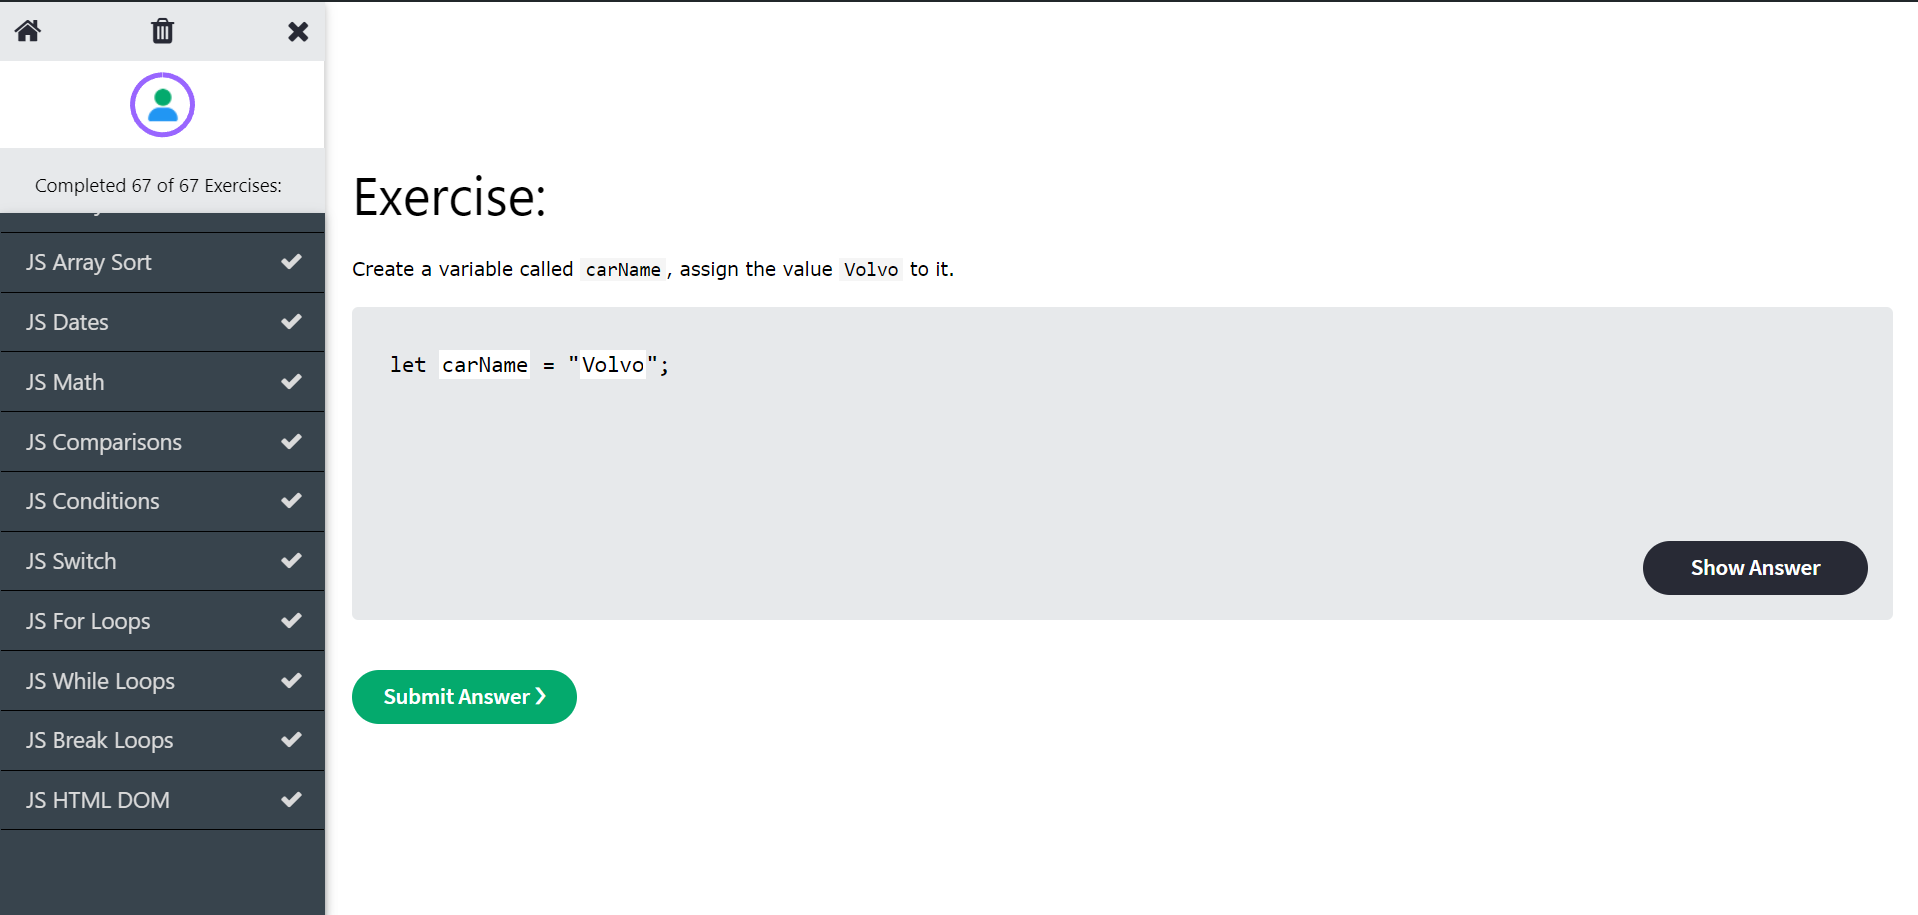
\includegraphics[width=1\textwidth,keepaspectratio]{img/EjerP2.png}
		\caption{Ejercicios - w3schools}
	\end{figure}
%%%%%%%%%%%%%%%%%%%%
    \subsection{Uso de GitHub : Creación de repositorio}
    
	\subsubsection{Cuenta de GitHub}
	\begin{figure}[H]
		\centering
		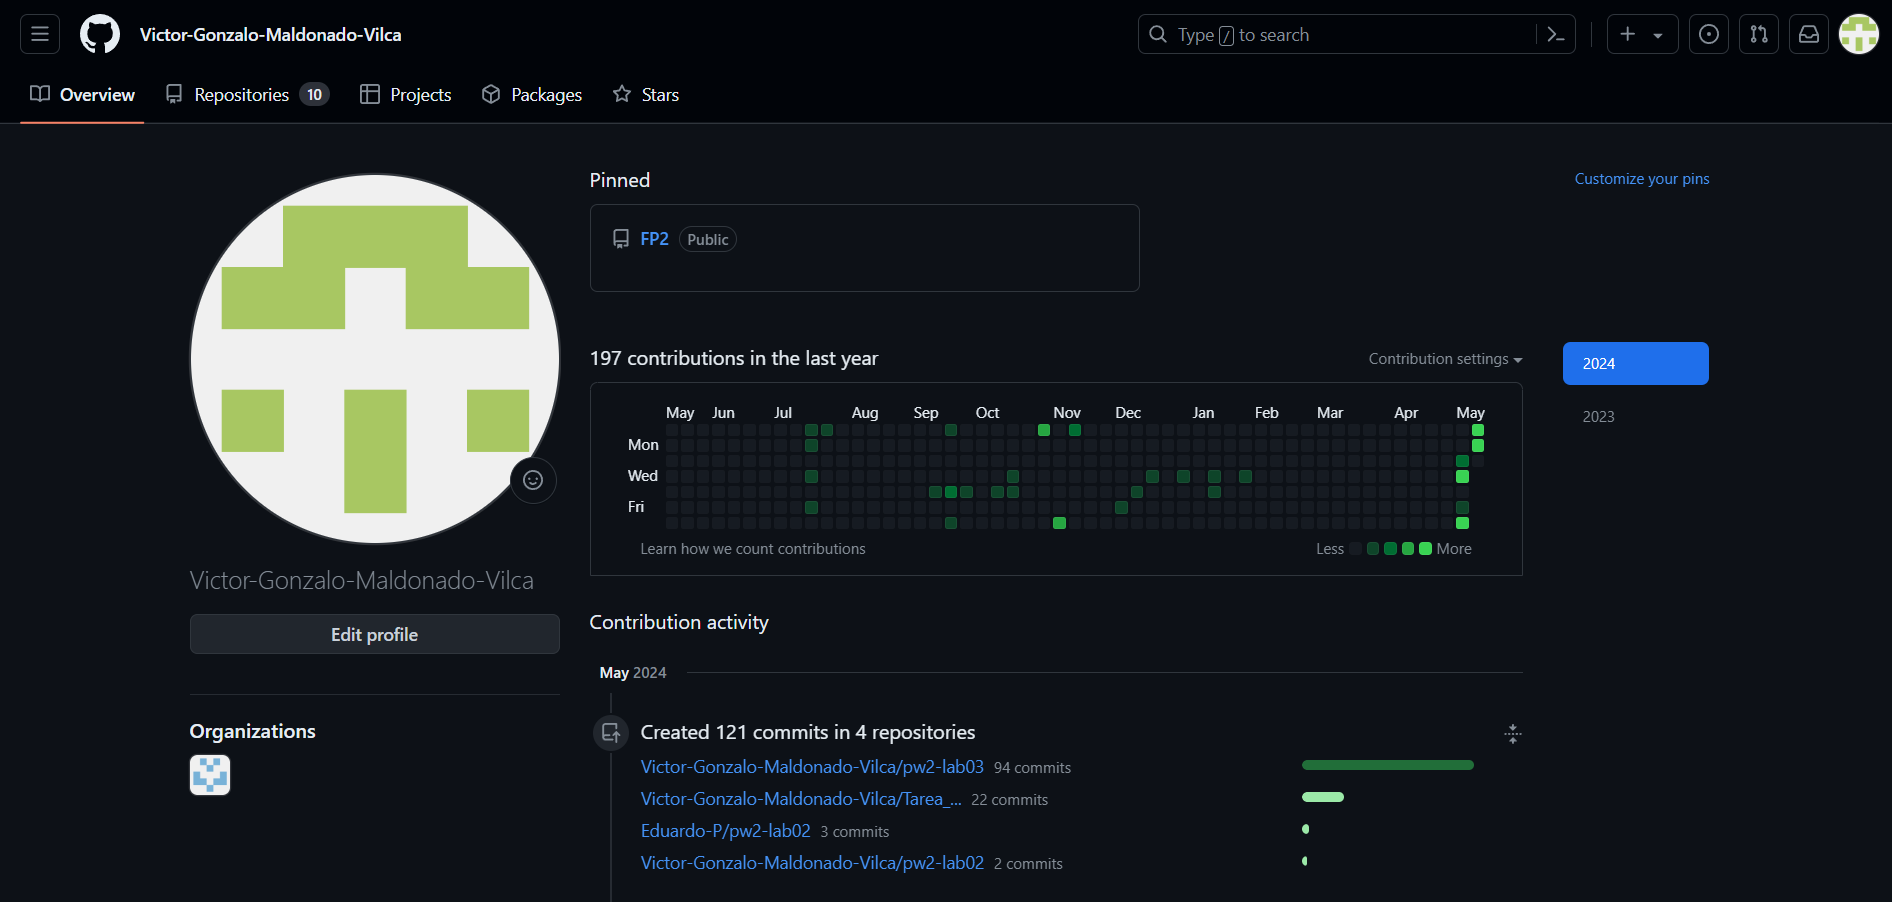
\includegraphics[width=0.87\textwidth,keepaspectratio]{img/usuario.png}
		\caption{Usuario}
	\end{figure}
%%%%%%%%%%%%%%%%%%%%
	\subsection{Creación de un Nuevo Repositorio}
	\subsubsection{Comandos}
	\begin{figure}[H]
		\centering
		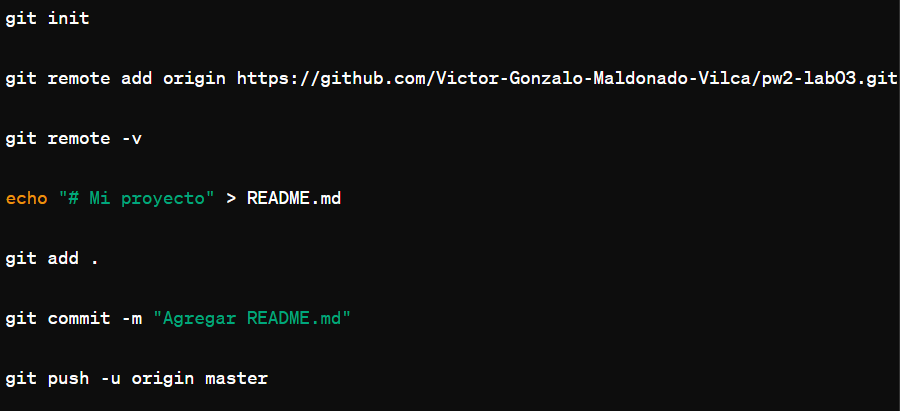
\includegraphics[width=0.9\textwidth,keepaspectratio]{img/Comandos_Iniciales.png}
		\caption{configuración inicial}
	\end{figure}
	\newpage
	\subsubsection{Implementación de Readme.md}
	\begin{figure}[H]
		\centering
		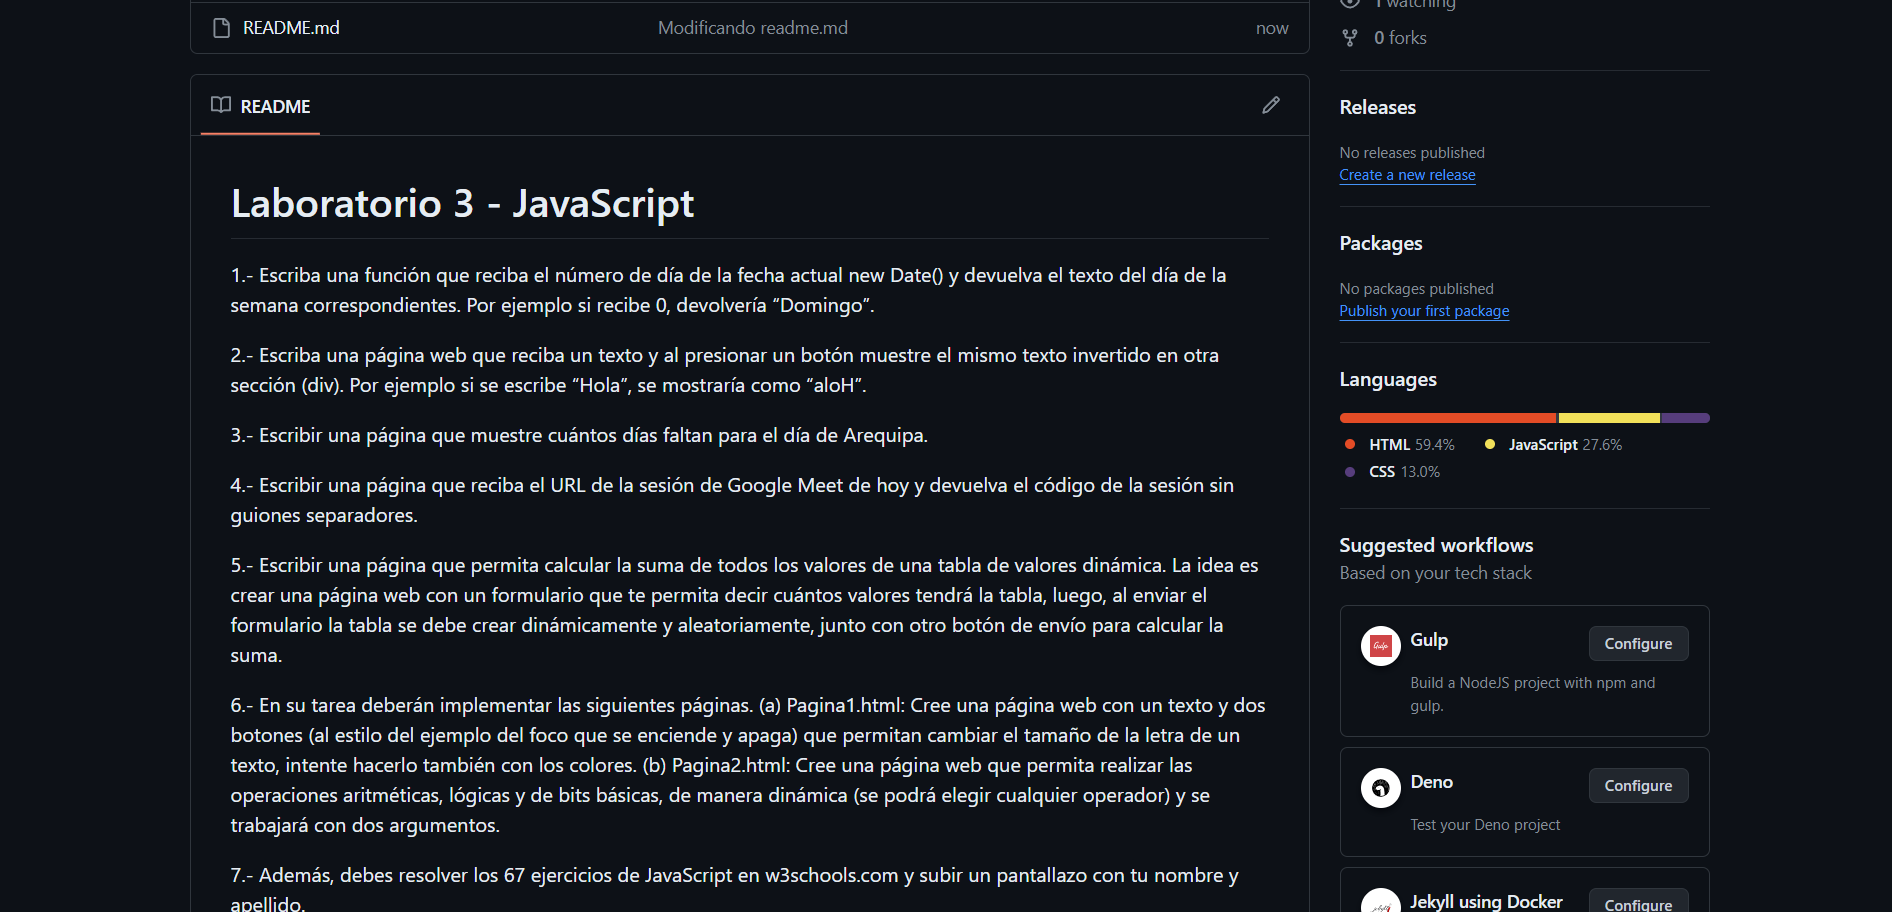
\includegraphics[width=0.9\textwidth,keepaspectratio]{img/readme.png}
		\caption{README.md}
	\end{figure}
%%%%%%%%%%%%%%%%%%%%
	\subsubsection{Registro de cambios en mi código}
	\begin{itemize}
		\item \textbf{Comandos}
		\begin{figure}[H]
			\centering
			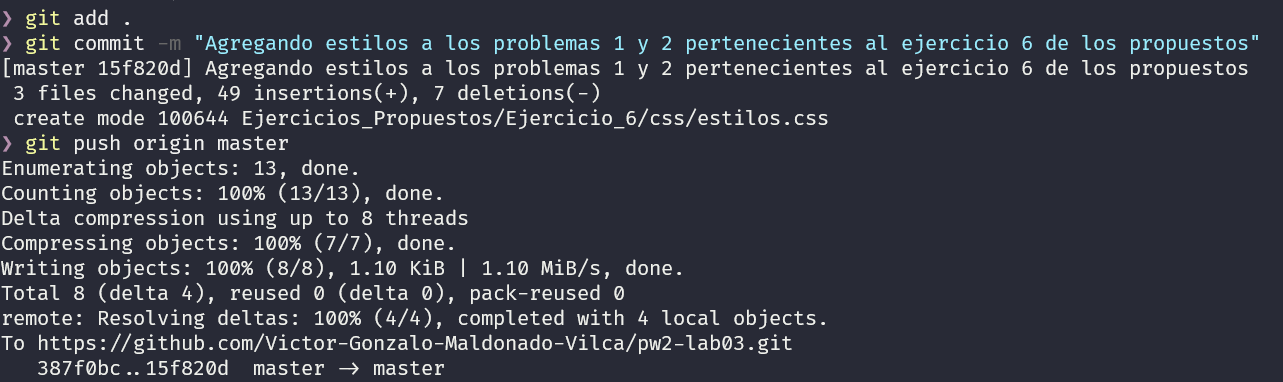
\includegraphics[width=0.95\textwidth,keepaspectratio]{img/Comandos.png}
			\caption{Comandos}
		\end{figure}
		\newpage
		\item \textbf{Commits}
		\begin{figure}[H]
			\centering
			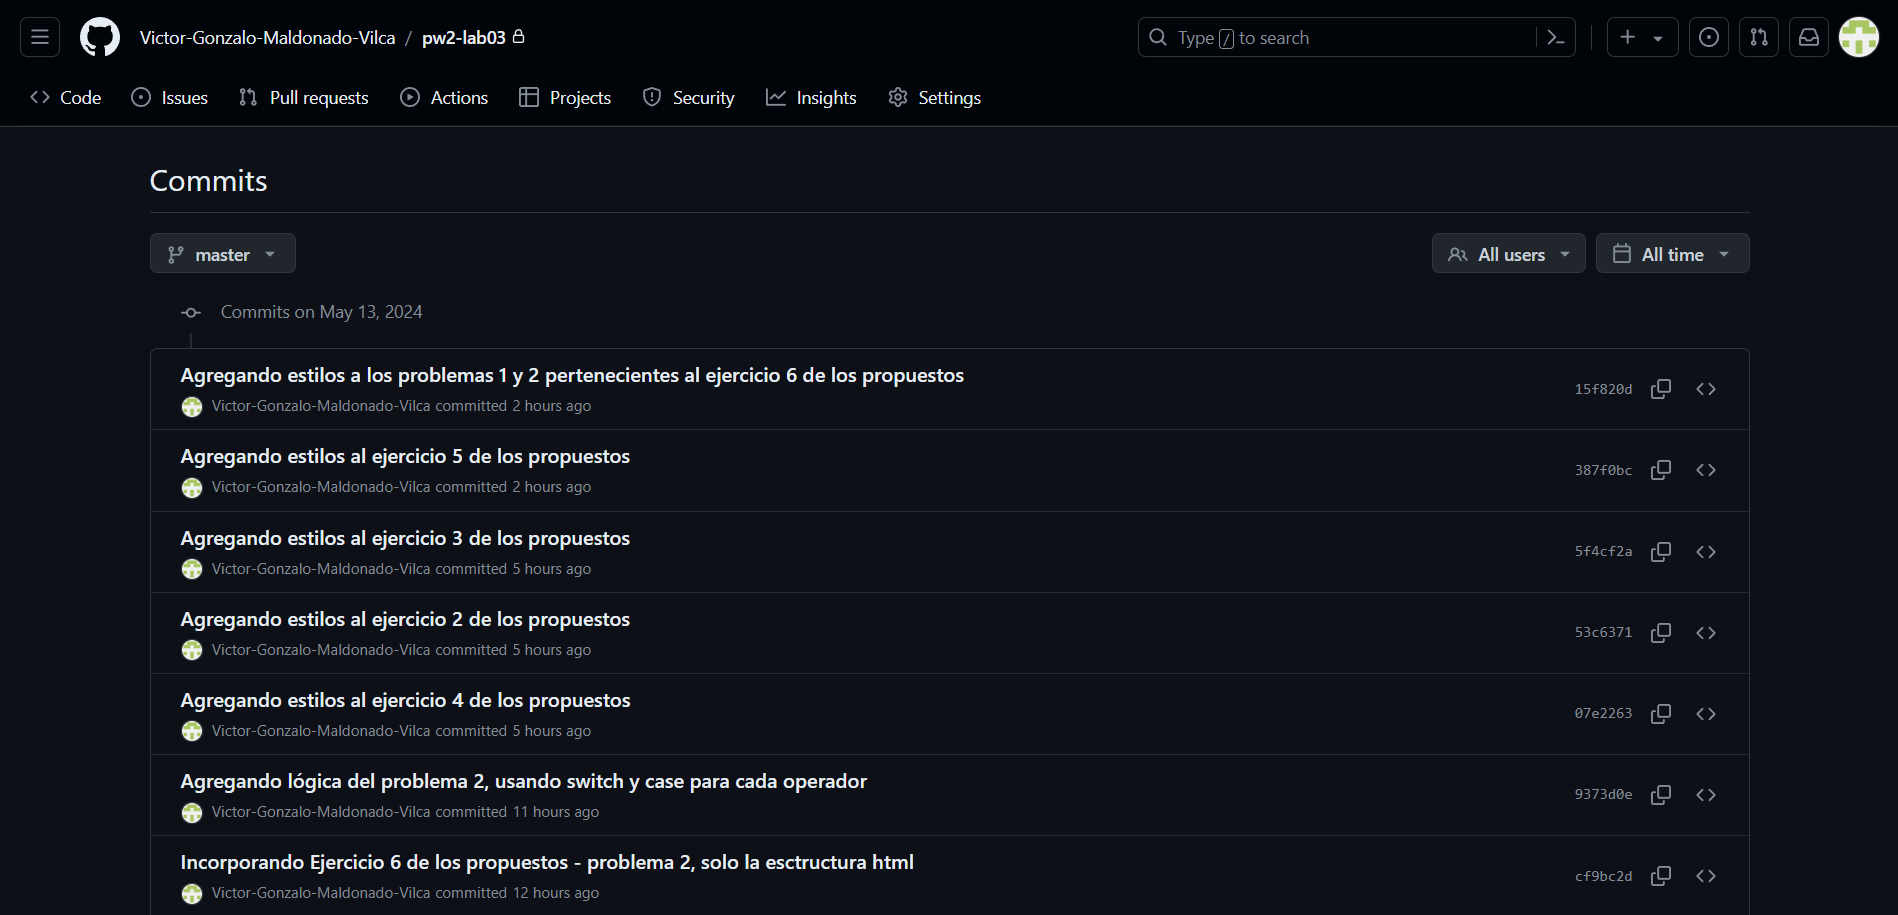
\includegraphics[width=0.94\textwidth,keepaspectratio]{img/Commits.png}
			\caption{Commits}
		\end{figure}
	\end{itemize}
	
%%%%%%%%%%%%%%%%%%%%
	\subsubsection{Repositorio}
	\begin{figure}[H]
		\centering
		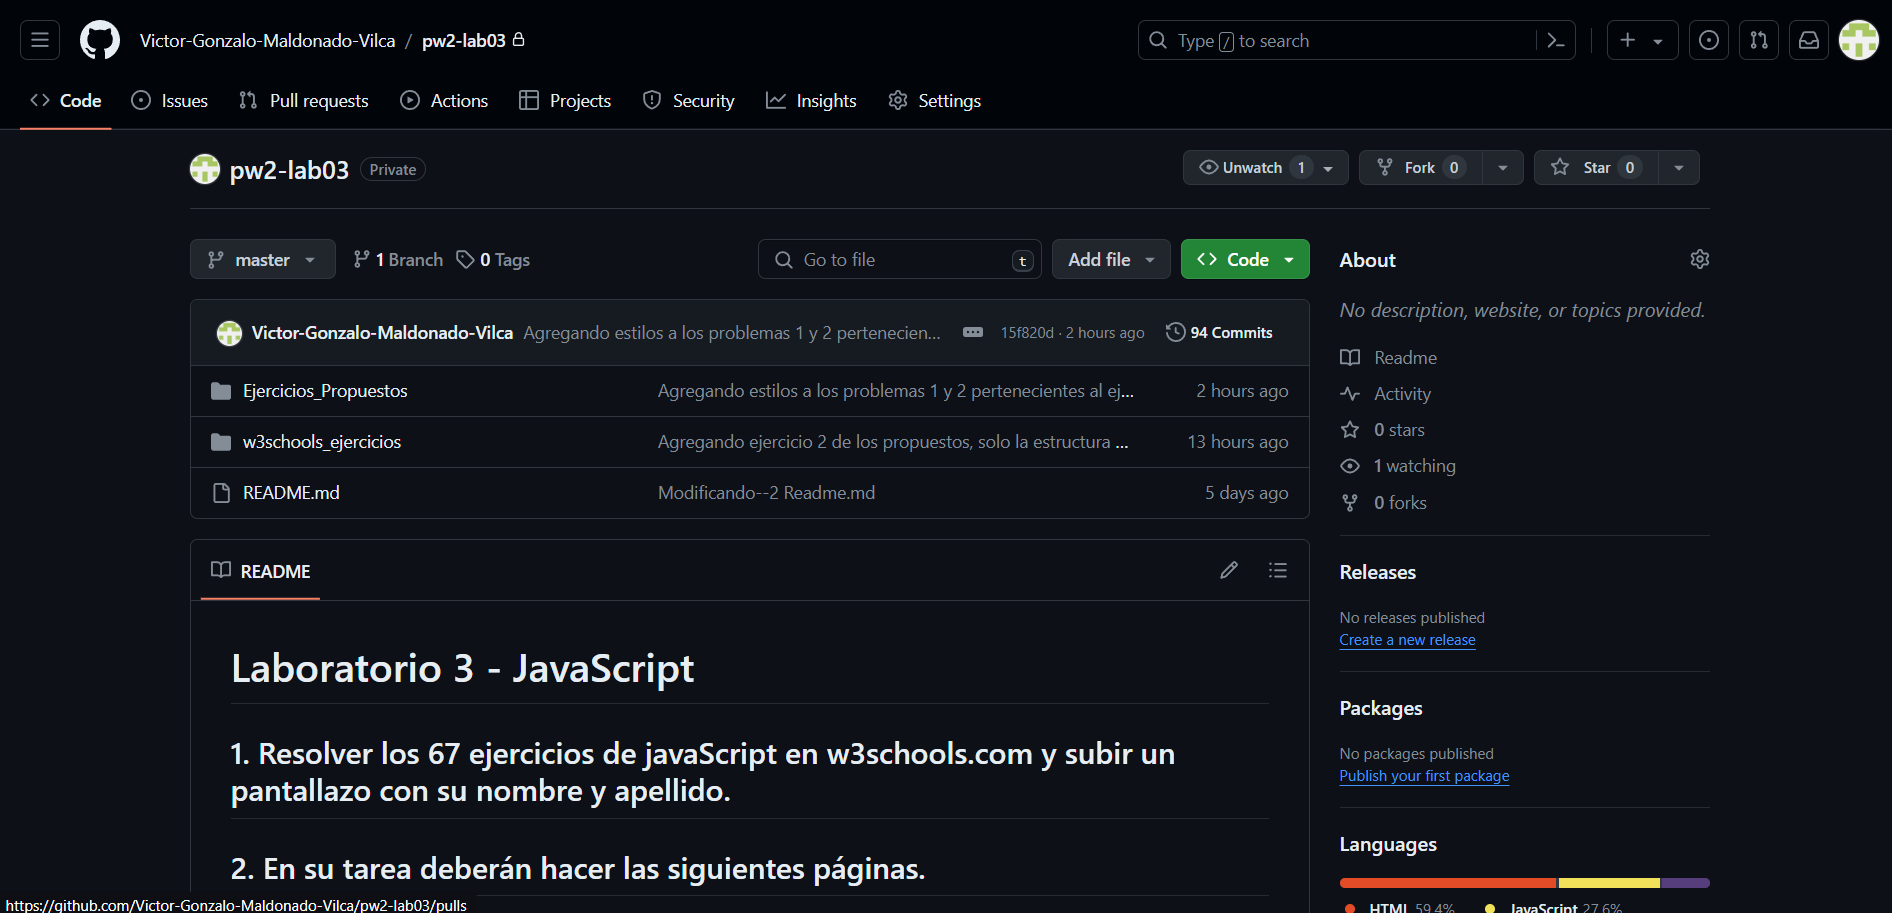
\includegraphics[width=1\textwidth,keepaspectratio]{img/Repositorio.png}
		\caption{Repositorio}
	\end{figure}
	\begin{figure}[H]
		\centering
		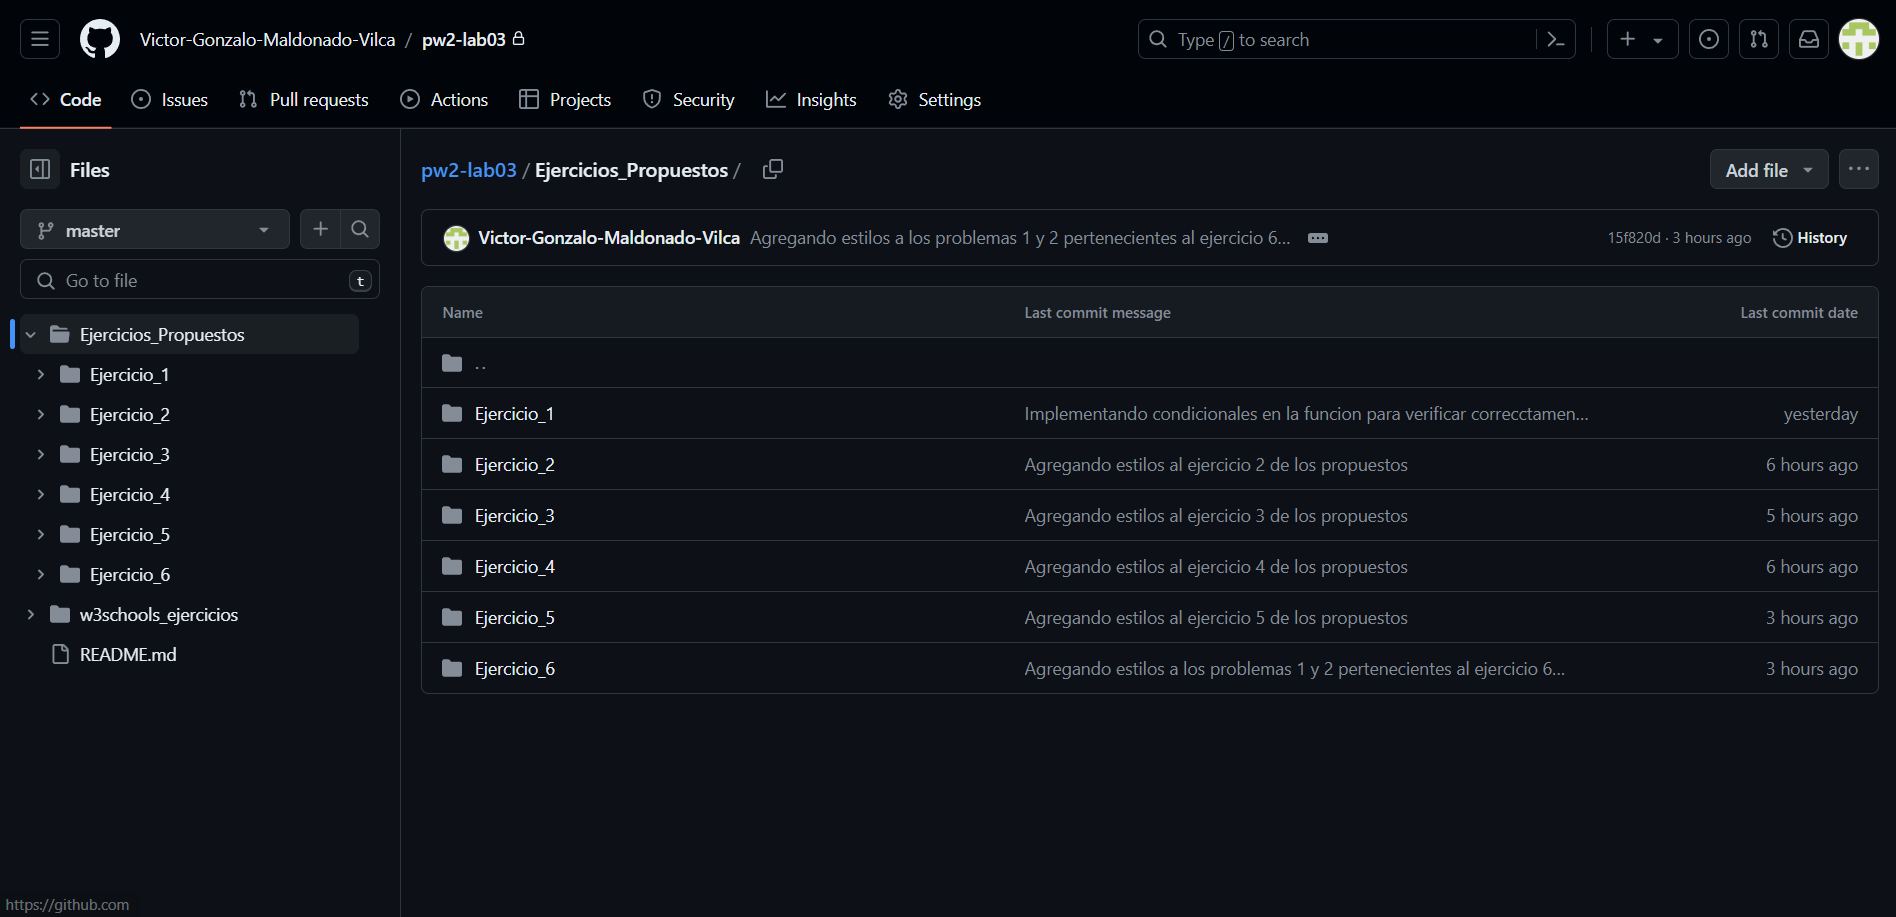
\includegraphics[width=1\textwidth,keepaspectratio]{img/Rep2.png}
		\caption{Repositorio - visualización}
	\end{figure}
%%%%%%%%%%%%%%%%%%%%
	\subsubsection{Proyecto compartido con el profesor de github}
	\begin{figure}[H]
		\centering
		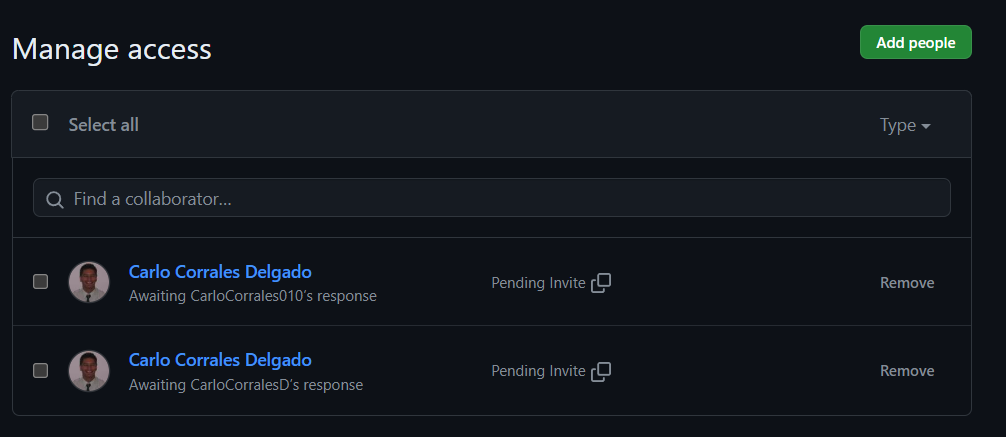
\includegraphics[width=1\textwidth,keepaspectratio]{img/Compartir.png}
		\caption{Compartir con el Profesor}
	\end{figure}
	\newpage
	\subsection{\textcolor{red}{Rúbrica para el contenido del Informe y demostración}}
	\begin{itemize}			
		\item El alumno debe marcar o dejar en blanco en celdas de la columna \textbf{Checklist} si cumplio con el ítem correspondiente.
		\item Si un alumno supera la fecha de entrega,  su calificación será sobre la nota mínima aprobada, siempre y cuando cumpla con todos lo items.
		\item El alumno debe autocalificarse en la columna \textbf{Estudiante} de acuerdo a la siguiente tabla:
	
		\begin{table}[ht]
			\caption{Niveles de desempeño}
			\begin{center}
			\begin{tabular}{ccccc}
    			\hline
    			 & \multicolumn{4}{c}{Nivel}\\
    			\cline{1-5}
    			\textbf{Puntos} & Insatisfactorio 25\%& En Proceso 50\% & Satisfactorio 75\% & Sobresaliente 100\%\\
    			\textbf{2.0}&0.5&1.0&1.5&2.0\\
    			\textbf{4.0}&1.0&2.0&3.0&4.0\\
    		\hline
			\end{tabular}
		\end{center}
	\end{table}	
	

	\end{itemize}

 
	
	\begin{table}[H]
		\caption{Rúbrica para contenido del Informe y demostración}
		\setlength{\tabcolsep}{0.5em} % for the horizontal padding
		{\renewcommand{\arraystretch}{1.5}% for the vertical padding
		%\begin{center}
		\begin{tabular}{|p{2.7cm}|p{7cm}|x{1.3cm}|p{1.2cm}|p{1.5cm}|p{1.1cm}|}
			\hline
    		\multicolumn{2}{|c|}{Contenido y demostración} & Puntos & Checklist & Estudiante & Profesor\\
			\hline
			\textbf{1. GitHub} & Hay enlace URL activo del directorio para el  laboratorio hacia su repositorio GitHub con código fuente terminado y fácil de revisar. &2 &X &2 & \\ 
			\hline
			\textbf{2. Commits} &  Hay capturas de pantalla de los commits más importantes con sus explicaciones detalladas. (El profesor puede preguntar para refrendar calificación). &4 &X &4 & \\ 
			\hline 
			\textbf{3. Código fuente} &  Hay porciones de código fuente importantes con numeración y explicaciones detalladas de sus funciones. &2 &X &2 & \\ 
			\hline 
			\textbf{4. Ejecución} & Se incluyen ejecuciones/pruebas del código fuente  explicadas gradualmente. &2 &X &2 & \\ 
			\hline			
			\textbf{5. Pregunta} & Se responde con completitud a la pregunta formulada en la tarea.  (El profesor puede preguntar para refrendar calificación).  &2 &X &2 & \\ 
			\hline	
			\textbf{6. Fechas} & Las fechas de modificación del código fuente estan dentro de los plazos de fecha de entrega establecidos. &2 &X &2 & \\ 
			\hline 
			\textbf{7. Ortografía} & El documento no muestra errores ortográficos. &2 &X &2 & \\ 
			\hline 
			\textbf{8. Madurez} & El Informe muestra de manera general una evolución de la madurez del código fuente,  explicaciones puntuales pero precisas y un acabado impecable.   (El profesor puede preguntar para refrendar calificación).  &4 &X &4 & \\ 
			\hline
			\multicolumn{2}{|c|}{\textbf{Total}} &20 & &20 & \\ 
			\hline
		\end{tabular}
		%\end{center}
		%\label{tab:multicol}
		}
	\end{table}


%%%%%%%%%%%%%%%%%%%%%%%%%%%%%%%%%%%%%%%%%%%%%%%%%%%%%%%%%%%%%%%%%%%
	\newpage
% 

    \section{Referencias}
    \begin{itemize}	
    	\item \url{https://www.w3schools.com/}
        \item \url{https://www.w3schools.com/js/exercise_js.asp?filename=exercise_js_variables1}
        \item \url{https://git-scm.com/doc}
	\end{itemize}

 
%\clearpage
%\bibliographystyle{apalike}
%\bibliographystyle{IEEEtranN}
%\bibliography{bibliography}
			
\end{document}